\documentclass[laboratorio]{guia}

\def \practnum {6} 
\def \practica {Ondas estacionarias en una cuerda}

\def \materia {Laboratorio de F\'\i sica II para Qu\'\i micos}
\def \periodo {2do. Cuatrimestre de 2015}
\def \catedra {Pablo Cobelli}
\def \website {http://materias.df.uba.ar/f2qa2015c2}
 
\usepackage{graphics}
\usepackage{amsmath}
\usepackage{amsfonts}
\usepackage{graphicx}
\usepackage{float}
\usepackage{wrapfig}
\usepackage{subfigure}
\usepackage{bm}
\usepackage{grffile}
\usepackage{color}
\usepackage{framed}
\usepackage[utf8]{inputenc}
\usepackage[T1]{fontenc}
\usepackage{lmodern}
\usepackage{circuitikz}
\usepackage[spanish]{babel}
\usepackage{babelbib}
\selectbiblanguage{spanish}

 

%----------------------------------------------------------
% Agrega al path de figuras el subdirectorio con el mismo
%     nombre que el archivo principal del proyecto
\graphicspath{{./\jobname/}}

%----------------------------------------------------------
% Definicion del entorno 'sabermas'
\makeatletter
\definecolor{shadecolor}{rgb}{0.89,0.91,0.94}
\newenvironment{sabermas}[1]{%
\vfill
\begin{shaded}
  \begin{center}
  {\textsection{Para saber m\'as}}
  \end{center}
  #1
\sf } 
{%
\end{shaded}%
}
\makeatother

%----------------------------------------------------------
% Definicion del entorno 'problema'
\newcounter{ContadorProblema}
\setcounter{ContadorProblema}{0}
\newcounter{TieneFiguraAsociada}
\setcounter{TieneFiguraAsociada}{0}
\newcounter{UbicacionFigura}
\setcounter{UbicacionFigura}{0}

\newenvironment{problema}[2][]
{%
    \ifx\relax#1\relax%
        \setcounter{TieneFiguraAsociada}{0}
        \else
        \setcounter{TieneFiguraAsociada}{1}
    \fi
    \def \archivofigura {#1}
    % 
    \refstepcounter{ContadorProblema}
    \noindent%
    \ifnum\value{TieneFiguraAsociada} < 1%
        {\sffamily \bfseries Problema \arabic{ContadorProblema}.}
        %{\sc {#1}}%
        \par\nobreak\par\nobreak%
        \medskip 
    \else
        % Va con figura; resta determinar de que lado.
        \ifnum\value{UbicacionFigura} < 1
            % Poner la figura del lado derecho
            \begin{minipage}{12.25cm}
            {\sffamily \bfseries Problema \arabic{ContadorProblema}.}
            %{\sc {#1}}%
            \par\nobreak\par\nobreak%
            \medskip 
        \else
            % Poner la figura del lado izquierdo
            \begin{minipage}{4.5cm}
                \centering
                \includegraphics[width=4.5cm]{\archivofigura}
                {\footnotesize {\sffamily Esquema asociado al 
                problema \arabic{ContadorProblema}}.}
            \end{minipage}\hfill%
            \begin{minipage}{12.25cm}
                {\sffamily \bfseries Problema \arabic{ContadorProblema}.}
                %{\sc {#1}}%
                \par\nobreak\par\nobreak%
                \medskip 
        \fi
    \fi
}
{%
    \ifnum\value{TieneFiguraAsociada} < 1%
        % \par \bigskip \vskip 0.3cm
    \else
        % Va con figura; resta determinar de que lado.
        \ifnum\value{UbicacionFigura} < 1
            % Poner la figura del lado derecho
            \end{minipage}\hfill%
            \begin{minipage}{4.5cm}
                \centering
                \includegraphics[width=4.5cm]{\archivofigura}
                {\footnotesize {\sffamily Esquema asociado al 
                problema \arabic{ContadorProblema}}.}
            \end{minipage}
        \else
            % Poner la figura del lado izquierdo
            \end{minipage}%
        \fi
    \fi
    \setcounter{TieneFiguraAsociada}{0}
    \par \bigskip \vskip 0.3cm
    % Permutamos el valor de la ubicacion
    \ifnum\value{UbicacionFigura} < 1
        \setcounter{UbicacionFigura}{1}
    \else
        \setcounter{UbicacionFigura}{0}
    \fi
}

%----------------------------------------------------------
% Definicion/Redefinicion de estilos
\renewcommand{\vec}[1]{\ensuremath{\mathbf{#1}}}



\hyphenation{ coe-fi-cien-tes coe-fi-cien-te au-to-va-lor
              au-to-va-lo-res co-rres-pon-der pro-ble-ma 
              cual-quie-ra po-la-ri-za-cio-nes }

\graphicspath{{./Guia_07_Ondas_en_una_cuerda/}}

\begin{document} 
\objetivo{%
    Realizar un estudio experimental de ondas estacionarias en cuerdas con sus
    dos extremos fijos. Se propone medir los modos normales de vibraci\'on,
    determinando experimentalmente sus frecuencias caracter\'\i sticas. En
    funci\'on de estos resultados, se busca determinar la velocidad de las
    ondas en t\'erminos de la tensi\'on y la densidad de masa de la cuerda.
    \tematicas{ondas estacionarias, ondas en una cuerda, modos normales,
frecuencias caracter\'\i sticas, velocidad de propagaci\'on.}} 
\maketitle

\section{Consideraciones preliminares}

La Figura~\ref{fig:1} muestra un esquema del dispositivo experimental propuesto
para el desarrollo de esta experiencia. En el mismo puede verse una cuerda (en
trazo azul grueso) sujeta en sus dos extremos. El extremo izquierdo est\'a fijo
a una pared (punto A), mientras que el extremo derecho est\'a fijo a una polea
(punto B). La distancia entre los puntos A y B es $L$. Vinculado 
mec\'anicamente con la cuerda, m\'as alla de la polea, se
encuentra un objeto de masa $m$, en reposo debido a la acci\'on combinada de la
gravedad y la tensi\'on provista por la cuerda. Cerca del punto A, un {\it
driver} mec\'anico imprime a la cuerda un movimiento oscilatorio arm\'onico de
frecuencia y amplitud controladas, provisto por un generador de funciones.

Para llevar a cabo la experiencia se dispone de una cuerda cuya masa por unidad de longitud $\mu$ puede
determinar experimentalmente. La tensi\'on mec\'anica que act\'ua
sobre la cuerda est\'a determinada por el peso colgado en uno de sus extremos,
seg\'un se observa en la Figura~\ref{fig:1}. 

La longitud de onda de cada modo excitado por el {\it driver} est\'a
determinada por la longitud de la cuerda, ya que la longitud $L$ es siempre
igual a un n\'umero entero de veces media longitud de onda.

Antes de continuar, aseg\'urese de poder responder estas dos preguntas:
\begin{itemize}
    \item ?`Por qu\'e vale $L = n (\lambda/2)$, siendo $n$ entero? 
    \item ?`C\'omo har\'\i a para conocer $\mu$ en sus condiciones de trabajo?
\end{itemize}


\section{Desarrollo de la experiencia}

\subsection{Primera parte}
Para un determinado valor de los par\'ametros $T$ y $\mu$, determine las
frecuencias $f$ para los primeros 8 modos normales de excitaci\'on de la
cuerda. Para cada uno de dichos modos, determine tambi\'en la longitud de onda
correspondiente $\lambda$ y, a partir de estos par\'ametros, calcule la
velocidad $v$ de la onda para cada modo. Grafique la velocidad de la onda en
funci\'on del orden de cada modo. ?`Qu\'e concluye a partir de sus resultados
experimentales?

\subsection{Segunda parte}

Para una cuerda dada, var\'\i e la masa $m$ colgada en uno de los extremos de
la cuerda. Para cada valor de $m$ empleado, determine la velocidad de la onda
en la cuerda. Tome al menos 8 valores de $m$. En cada caso, determine el valor
de $T$ y $\mu$. Grafique entonces $v$ en funci\'on de $\sqrt{T/\mu}$. ?`Qu\'e
conclusi\'on puede obtener en este caso?

\begin{figure}[t!]
    \centering
    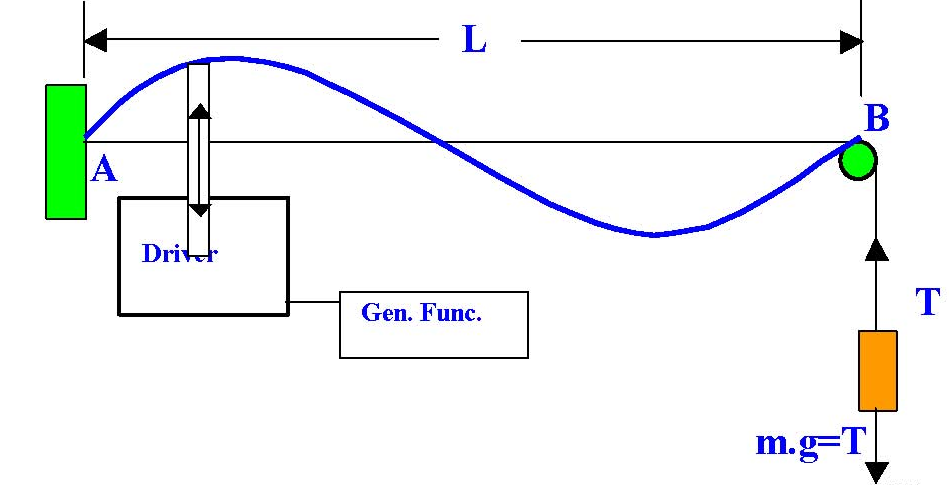
\includegraphics[width=8.5cm]{LG07--004.png}
    \caption{Esquema del montaje experimental propuesto para la realizaci\'on
    de esta pr\'actica.}
    \label{fig:1}
\end{figure}

\subsection{Tercera parte}

Cuando var\'\i a la masa $m$, se var\'\i a tanto la tensi\'on $T$ como la
densidad de masa $m$. Demuestre que la relaci\'on entre la velocidad de la onda
y la masa $m$ colgada es:
\begin{equation}
    v = \sqrt{\frac{m (L_0 + k m)g}{m_c}},
    \label{eq:1}
\end{equation}
donde $m_c$ es la masa total de la cuerda, $L_0$ su longitud natural y $k$ la
constante de estiramiento de la cuerda. ?`C\'omo puede determinar el valor de $k$
experimentalmente? Discuta su idea con el docente y lleve adelante la
medici\'on de $k$. Luego compare en un gr\'afico la relaci\'on encontrada
experimentalmente entre $v$ y $m$; y en el mismo gr\'afico indique la curva que
esperar\'\i a te\'oricamente para esta relaci\'on usando la ecuaci\'on
\eqref{eq:1}. Describa sus conclusiones en este caso.



\nocite{Alonso1998,Crawford1994}
\bibliographystyle{unsrt} 
\bibliography{Bibliografia}


\end{document}
